% Embedded bibliography. On first compile this writes arp.bib to disk.
% Then run: bibtex <jobname>; pdflatex; pdflatex (as usual).
\begin{filecontents*}[overwrite]{arp.bib}
@incollection{ClarkBrennan1991,
  author    = {Clark, Herbert H. and Brennan, Susan E.},
  title     = {Grounding in communication},
  booktitle = {Perspectives on Socially Shared Cognition},
  editor    = {Resnick, Lauren B. and Levine, John M. and Teasley, Stephanie D.},
  publisher = {American Psychological Association},
  address   = {Washington, DC},
  year      = {1991},
  pages     = {127--149},
}

@article{ClarkSchaefer1989,
  author  = {Clark, Herbert H. and Schaefer, Edward F.},
  title   = {Contributing to discourse},
  journal = {Cognitive Science},
  volume  = {13},
  number  = {2},
  pages   = {259--294},
  year    = {1989},
}

@article{Gisladottir2015,
  author  = {Gisladottir, Rosa S. and Chwilla, Dorothee J. and Levinson, Stephen C.},
  title   = {Conversation electrified: {ERP} correlates of speech act recognition in underspecified utterances},
  journal = {PLOS ONE},
  volume  = {10},
  number  = {3},
  pages   = {e0120068},
  year    = {2015},
}

@book{Givon1983,
  editor    = {Giv{\'o}n, Talmy},
  title     = {Topic Continuity in Discourse: A Quantitative Cross-Language Study},
  publisher = {John Benjamins},
  address   = {Amsterdam},
  year      = {1983},
}

@article{Garrod2007,
  author  = {Garrod, Simon and Pickering, Martin J.},
  title   = {Automaticity of language production in monologue and dialogue},
  journal = {Trends in Cognitive Sciences},
  volume  = {11},
  number  = {1},
  pages   = {1--2},
  year    = {2007},
}

@article{HancockRubin2015,
  author  = {Hancock, Adrienne B. and Rubin, Benjamin A.},
  title   = {Influence of communication partner's gender on language},
  journal = {Journal of Language and Social Psychology},
  volume  = {34},
  number  = {1},
  pages   = {46--64},
  year    = {2015},
}

@book{Hayashi2003,
  author    = {Hayashi, Makoto},
  title     = {Joint Utterance Construction in {Japanese} Conversation},
  publisher = {John Benjamins},
  address   = {Amsterdam},
  year      = {2003},
}

@article{Helasvuo2004,
  author  = {Helasvuo, Marja-Liisa},
  title   = {Shared syntax: The grammar of co-constructions},
  journal = {Journal of Pragmatics},
  volume  = {36},
  number  = {8},
  pages   = {1315--1336},
  year    = {2004},
}

@incollection{HeritageWatson1979,
  author    = {Heritage, John and Watson, D. Rod},
  title     = {Formulations as conversational objects},
  booktitle = {Everyday Language: Studies in Ethnomethodology},
  editor    = {Psathas, George},
  publisher = {Irvington},
  address   = {New York},
  year      = {1979},
  pages     = {123--162},
}

@article{HollerKendrick2015,
  author  = {Holler, Judith and Kendrick, Kobin H.},
  title   = {Unaddressed participants' gaze in multi-person interaction: Optimizing recipiency},
  journal = {Frontiers in Psychology},
  volume  = {6},
  pages   = {98},
  year    = {2015},
}

@article{Itakura2001,
  author  = {Itakura, Hiroko},
  title   = {Describing conversational dominance},
  journal = {Journal of Pragmatics},
  volume  = {33},
  number  = {12},
  pages   = {1859--1880},
  year    = {2001},
}

@article{JacksonMarsh1996,
  author  = {Jackson, Susan A. and Marsh, Herbert W.},
  title   = {Development and validation of a scale to measure optimal experience: The {Flow State Scale}},
  journal = {Journal of Sport and Exercise Psychology},
  volume  = {18},
  number  = {1},
  pages   = {17--35},
  year    = {1996},
}

@article{Kim2003,
  author  = {Kim, Kyu-hyun},
  title   = {An analysis of collaborative completion in {Korean} conversation},
  journal = {Language Research},
  volume  = {39},
  number  = {1},
  pages   = {147--182},
  year    = {2003},
}

@article{KoschmannLeBaron2003,
  author  = {Koschmann, Timothy and LeBaron, Curtis},
  title   = {Reconsidering common ground: Examining {Clark}'s contribution theory in the {OR}},
  journal = {ECSCW 2003: Proceedings of the Eighth European Conference on Computer Supported Cooperative Work},
  pages   = {81--98},
  year    = {2003},
}

@article{Lerner1991,
  author  = {Lerner, Gene H.},
  title   = {On the syntax of sentences-in-progress},
  journal = {Language in Society},
  volume  = {20},
  number  = {3},
  pages   = {441--458},
  year    = {1991},
}

@incollection{Lerner1996,
  author    = {Lerner, Gene H.},
  title     = {On the ``semi-permeable'' character of grammatical units in conversation: Conditional entry into the turn space of another speaker},
  booktitle = {Interaction and Grammar},
  editor    = {Ochs, Elinor and Schegloff, Emanuel A. and Thompson, Sandra A.},
  publisher = {Cambridge University Press},
  address   = {Cambridge},
  year      = {1996},
  pages     = {238--276},
}

@article{Levinson2016,
  author  = {Levinson, Stephen C.},
  title   = {Turn-taking in human communication: Origins and implications for language processing},
  journal = {Trends in Cognitive Sciences},
  volume  = {20},
  number  = {1},
  pages   = {6--14},
  year    = {2016},
}

@article{Linell1988,
  author  = {Linell, Per and Gustavsson, Lennart and Juvonen, P{\"a}ivi},
  title   = {Interactional dominance in dyadic communication: A presentation of initiative-response analysis},
  journal = {Linguistics},
  volume  = {26},
  number  = {3},
  pages   = {415--442},
  year    = {1988},
}

@article{Liu2017,
  author  = {Liu, Ning and Mok, Cindy and Witt, Emily E. and Pradhan, Aarti H. and Chen, Jingyuan E. and Reiss, Allan L.},
  title   = {{NIRS}-based hyperscanning reveals inter-brain neural synchronization during cooperative {Jenga} game with face-to-face communication},
  journal = {Frontiers in Human Neuroscience},
  volume  = {11},
  pages   = {82},
  year    = {2017},
}

@article{MagyariDeRuiter2012,
  author  = {Magyari, Lilla and de Ruiter, Jan P.},
  title   = {Prediction of turn-ends based on anticipation of upcoming words},
  journal = {Frontiers in Psychology},
  volume  = {3},
  pages   = {376},
  year    = {2012},
}

@article{PickeringGarrod2004,
  author  = {Pickering, Martin J. and Garrod, Simon},
  title   = {Toward a mechanistic psychology of dialogue},
  journal = {Behavioral and Brain Sciences},
  volume  = {27},
  number  = {2},
  pages   = {169--225},
  year    = {2004},
}

@article{PickeringGarrod2013,
  author  = {Pickering, Martin J. and Garrod, Simon},
  title   = {An integrated theory of language production and comprehension},
  journal = {Behavioral and Brain Sciences},
  volume  = {36},
  number  = {4},
  pages   = {329--347},
  year    = {2013},
}

@article{Riest2015,
  author  = {Riest, Carina and Jorschick, Annett B. and de Ruiter, Jan P.},
  title   = {Anticipation in turn-taking: Mechanisms and information sources},
  journal = {Frontiers in Psychology},
  volume  = {6},
  pages   = {89},
  year    = {2015},
}

@article{Sacks1974,
  author  = {Sacks, Harvey and Schegloff, Emanuel A. and Jefferson, Gail},
  title   = {A simplest systematics for the organization of turn-taking for conversation},
  journal = {Language},
  volume  = {50},
  number  = {4},
  pages   = {696--735},
  year    = {1974},
}

@incollection{Schegloff1982,
  author    = {Schegloff, Emanuel A.},
  title     = {Discourse as an interactional achievement: Some uses of ``uh huh'' and other things that come between sentences},
  booktitle = {Analyzing Discourse: Text and Talk},
  editor    = {Tannen, Deborah},
  publisher = {Georgetown University Press},
  address   = {Washington, DC},
  year      = {1982},
  pages     = {71--93},
}

@article{Stephens2010,
  author  = {Stephens, Greg J. and Silbert, Lauren J. and Hasson, Uri},
  title   = {Speaker-listener neural coupling underlies successful communication},
  journal = {Proceedings of the National Academy of Sciences},
  volume  = {107},
  number  = {32},
  pages   = {14425--14430},
  year    = {2010},
}

@article{Stivers2009,
  author  = {Stivers, Tanya and Enfield, N. J. and Brown, Penelope and Englert, Christina and Hayashi, Makoto and Heinemann, Trine and Hoymann, Gertie and Rossano, Federico and de Ruiter, Jan P. and Yoon, Kyung-Eun and Levinson, Stephen C.},
  title   = {Universals and cultural variation in turn-taking in conversation},
  journal = {Proceedings of the National Academy of Sciences},
  volume  = {106},
  number  = {26},
  pages   = {10587--10592},
  year    = {2009},
}

@incollection{WestZimmerman1983,
  author    = {West, Candace and Zimmerman, Don H.},
  title     = {Small insults: A study of interruptions in cross-sex conversations between unacquainted persons},
  booktitle = {Language, Gender and Society},
  editor    = {Thorne, Barrie and Kramarae, Cheris and Henley, Nancy},
  publisher = {Newbury House},
  address   = {Rowley, MA},
  year      = {1983},
  pages     = {102--117},
}

@incollection{ZimmermanWest1975,
  author    = {Zimmerman, Don H. and West, Candace},
  title     = {Sex roles, interruptions and silences in conversation},
  booktitle = {Language and Sex: Difference and Dominance},
  editor    = {Thorne, Barrie and Henley, Nancy},
  publisher = {Newbury House},
  address   = {Rowley, MA},
  year      = {1975},
  pages     = {105--129},
}
\end{filecontents*}

% Standalone single-file build of the ARP paper.
% Bibliography is embedded above via filecontents*.
% Build: pdflatex -> bibtex -> pdflatex x2.
\documentclass[11pt,letterpaper]{article}
\usepackage[margin=1in]{geometry}
\usepackage{setspace}
\usepackage{microtype}
\usepackage{titlesec}
\usepackage{enumitem}
\usepackage{parskip}
\usepackage[hidelinks]{hyperref}
\usepackage{tikz}
\usetikzlibrary{arrows.meta,positioning,calc}
\usepackage{natbib}
\bibliographystyle{apalike}

\titleformat{\section}{\normalfont\large\bfseries}{\thesection}{0.7em}{}
\titleformat{\subsection}{\normalfont\normalsize\bfseries}{\thesubsection}{0.7em}{}
\titleformat{\paragraph}[runin]{\normalfont\normalsize\bfseries}{}{0pt}{}[.]

\setlength{\parindent}{0pt}
\setlength{\parskip}{0.6em}
\onehalfspacing

\title{\textbf{The Assimilate--Receipt--Pivot:\\A Constitutive Mechanism of Conversation}}
\author{Daryl Janzen\\\small Department of Physics and Engineering Physics\\\small University of Saskatchewan}
\date{}

\begin{document}
\maketitle


\noindent\textbf{Abstract.} This article advances a constitutive theory of conversation. I argue that conversation, as distinct from related communicative activities such as lecture, monologue, ritual exchange, and parallel speech, is constituted by the exchange of a single conversational move with three structural components: \emph{assimilate}, \emph{receipt}, and \emph{pivot} (ARP). The current listener assimilates the prior speaker's contribution sufficiently to ground a public formulation (the receipt), then extends the inferential chain by introducing new content the assimilation made available (the pivot). I argue that the three steps are mutually constitutive rather than co-occurring, and that this integration consolidates findings currently distributed across four research traditions: turn-taking and projection, collaborative completion, interactive alignment, and grounding. The construct organises a two-axis space in which conversational moves are located. The first axis is \emph{participation}, signed from anti-conversational (active termination and inversion of the ARP contract) through non-conversational (activity that does not engage the contract) to conversational (positive engagement). The second axis is \emph{quality} ($Q$), continuous and indexing the degree to which the three steps are compressed---temporally, cognitively, or in surface form. High-$Q$ moves include pre-emptive receipts of in-progress content, succinct crystallisations that name a partner's point more clearly than the partner had it themselves, and generative pivots that open inferential territory neither speaker had explicitly reached. The standard phenomenology of conversation---fluency, ``flow,'' being on the same wavelength, talking past each other, being talked at, being shut down---sorts into this two-axis space in ways that flat theories of dialogic processing do not predict. I distinguish ARPs from collaborative completion, backchannelling, formulation, and intrusive interruption; consider whether the construct can be reduced to any single parent theory and argue that it cannot; derive predictions about both axes; and outline a methodological programme.

\medskip
\noindent\textit{Keywords:} turn-taking, projection, collaborative completion, interactive alignment, grounding, conversational dominance, conversational flow


\section{Introduction}

\subsection{What is conversation?}

We have separate words for activities that involve two or more people speaking in alternation. We call some of them conversations and others lectures, monologues, rituals, interrogations, arguments, performances, negotiations, briefings, and so on. The folk taxonomy is not idle: speakers reliably distinguish a conversation from a lecture even when both involve roughly equal speaking time, and reliably distinguish a conversation from parallel monologue even when both consist of fluent alternation. Something is being tracked beyond the surface form of speech alternation, and the question of what it is has not been satisfactorily answered.

The dominant theoretical traditions in this area each describe a feature of successful dialogue without claiming to define the activity. Conversation Analysis describes the turn-taking system \citep{Sacks1974} and a family of embedded practices including projection, repair, and collaborative completion \citep{Lerner1991,Hayashi2003}. The interactive-alignment account in psycholinguistics describes how interlocutors' mental representations converge \citep{PickeringGarrod2004,PickeringGarrod2013}. The contribution model describes how utterances are grounded through demonstrated uptake \citep{ClarkSchaefer1989,ClarkBrennan1991}. The sociolinguistic literature on conversational dominance describes how violations of turn-taking rights produce withdrawal in the disadvantaged party \citep{ZimmermanWest1975,WestZimmerman1983,Itakura2001}. Each tradition has accumulated substantial empirical support, and each treats its target phenomenon as a feature of dialogue rather than as its definition.

This article advances a different proposal. I argue that conversation is constituted by the exchange of a single move---the Assimilate--Receipt--Pivot (ARP)---and that the activities we have separate names for are activities in which ARP-exchange is absent, suppressed, inverted, or replaced by something else. The phenomenology of fluent conversation is the phenomenology of high-quality ARP-exchange. The phenomenology of being talked at is the phenomenology of being structurally denied opportunities to ARP. The phenomenology of being shut down is the phenomenology of having an ARP-exchange terminated by a move directed against the contract itself. Conversation, on this account, is not a thing that sometimes has ARP-exchange in it; it is the activity of ARP-exchange.

\subsection{The Assimilate--Receipt--Pivot}

An ARP, informally, is a floor-taking move with three structural components. The current listener \emph{assimilates} the prior speaker's contribution sufficiently to ground a public formulation. The opening of the listener's turn delivers that formulation as a \emph{receipt}: a demonstration of understanding in the listener's own terms. The continuation of the turn \emph{pivots} to a new contribution that the assimilation made available, extending the inferential chain.

The three components are not phases of separate cognitive operations; they are descriptions of a single cognitive--interactional event. The act of assimilating the speaker's contribution is what produces both the formulation deployed in the receipt and the extension deployed in the pivot. The receipt and pivot are joined at a structural location: the receipt completes the prior speaker's contribution and thereby vacates the floor for the pivot, which uses the assimilated material as its launching point.

I argue in Section~\ref{sec:construct} that this integration is what the parent literatures, severally, do not articulate, and that the integration is structurally necessary rather than incidental.

\subsection{The two-axis structure}

Once conversation is identified with ARP-exchange, conversational moves can be located in a two-axis space.

The first axis is \emph{participation}, which is signed. Positive participation is engagement in the ARP contract: producing ARPs, inviting them, ratifying them, or producing other moves (questions, openings, repairs) that maintain the contract. Zero participation is non-conversational activity that doesn't engage the contract: lecture, recitation, ritualised greeting, talking to oneself in a partner's presence. Negative participation is moves directed against the contract: ``stop talking,'' the calibrated non-receipt to a vulnerable disclosure, walking out mid-sentence, deliberate floor-monopolisation. Negative-participation moves presuppose the contract in order to attack it, and are therefore structurally distinct from zero-participation activity, which simply doesn't engage it.

The second axis is \emph{quality}, denoted $Q$, and is continuous and positive. $Q$ indexes the degree to which the three components of an ARP are \emph{compressed}: temporally, cognitively, or in surface form. Low-$Q$ ARPs unfold the three steps sequentially with little overlap and at full length. High-$Q$ ARPs compress the steps in various ways: the receipt may be pre-emptive, formulating content the prior speaker has not yet uttered, so that the assimilation step skips ahead and the prior speaker's continued articulation becomes redundant. The receipt may be unusually succinct, crystallising a complex contribution into a clause that the prior speaker recognises as more precise than what they had themselves. The pivot may be generative, opening inferential territory the prior speaker had not yet reached. In the highest-$Q$ limit, the three components zipper-merge into a single flow: an outside listener has difficulty parsing whose contribution is whose at any given instant, and the seam between the two speakers becomes inaudible. The standard phenomenology of ``flow,'' ``vibing,'' and ``being on the same wavelength'' is the felt experience of sustained high-$Q$ ARP-exchange.

The two axes are orthogonal. They tend to covary in practice---sincere participation supports the model-building that high $Q$ requires, and high $Q$ rewards continued participation---but the cases that violate this covariance are diagnostic. Section~\ref{sec:plane} develops the two-axis structure in detail and uses several off-diagonal cases to show that the axes are genuinely distinct.

\subsection{Plan of the article}

Section~\ref{sec:background} reviews the four parent literatures and identifies what each contributes to the present synthesis and where each is silent. Section~\ref{sec:construct} specifies the ARP construct and argues for the structural necessity of the integration. Section~\ref{sec:plane} introduces the two-axis structure and uses it to locate the standard conversational phenomenology. Section~\ref{sec:against} considers whether the ARP can be reduced to any single parent theory and argues that it cannot. Section~\ref{sec:predictions} derives predictions about both axes. Section~\ref{sec:methods} outlines a methodological programme. Section~\ref{sec:discussion} considers limitations and theoretical implications.

\section{The Four Parent Literatures}\label{sec:background}

\subsection{Projection and the turn-taking system}

\citet{Sacks1974} showed that conversational turns are constructed out of turn-constructional units (TCUs) whose syntactic, prosodic, and pragmatic shape allows listeners to project the location of a possible completion---the transition-relevance place (TRP). The empirical literature has confirmed that projection rather than reaction underlies turn timing: \citet{Riest2015} showed that the distribution of estimated turn ends in natural turns matches the distribution obtained under full advance information; \citet{MagyariDeRuiter2012} showed that anticipation tracks upcoming words; \citet{HollerKendrick2015} extended the finding to gaze orientation in multi-party settings.

Critically, projection extends beyond timing to content. \citet{Gisladottir2015} provided neural evidence that listeners anticipate not only when a turn will end but what kind of action it will perform. Projection includes prediction of the inferential trajectory of an unfolding turn, not merely its boundary. The ARP construct is licensed by this fact: projection is what makes pre-emptive assimilation possible, which in turn makes high-$Q$ receipts and pivots available.

The Conversation Analysis literature has not theorised a single move in which assimilation, demonstration of assimilation, and extension of the inferential chain are jointly performed. Anticipatory completion \citep{Lerner1991,Lerner1996,Hayashi2003} approaches this move but stops short of the pivot, as I discuss in Section~\ref{sec:construct}.

\subsection{Collaborative completion and co-constructed syntax}

\citet{Lerner1991} identified a family of practices in which one speaker syntactically and semantically completes a TCU begun by another. \citet{Hayashi2003} documented analogous structures in Japanese; \citet{Helasvuo2004} developed the construct of \emph{shared syntax}; \citet{Kim2003} extended the analysis to Korean.

Collaborative completion has been analysed primarily as a syntactic--interactional achievement. Its function as evidence of assimilation has been noted but rarely treated as central. The ARP construct treats the evidential function---demonstration of accurate assimilation---as primary, with the syntactic continuation as one surface expression of an underlying cognitive event.

\subsection{Interactive alignment}

\citet{PickeringGarrod2004} proposed that successful dialogue depends on the alignment of mental representations across multiple linguistic levels, with alignment cascading from low-level phonetic and lexical levels to higher-level situation models via automatic priming. The 2013 refinement incorporated forward models, such that alignment partly consists in matching predictions about upcoming material \citep{PickeringGarrod2013}.

The interactive-alignment account has two relevant silences. First, priming-based alignment is largely automatic and not directly observable to interlocutors; some additional, surface-level evidence is required for partners to mutually believe that alignment has been achieved. Second, the account models alignment as a continuous, gradient property of the dialogic state without picking out specific moves at which alignment is publicly verified. The ARP is proposed as the move at which exactly this verification occurs.

\subsection{Grounding and the contribution model}

\citet{ClarkSchaefer1989} and \citet{ClarkBrennan1991} developed the contribution model, in which each contribution proceeds through a presentation phase and an acceptance phase. The grounding criterion is met when both participants mutually believe that the contribution has been understood to a criterion sufficient for current purposes. Demonstrations of understanding---next-turn proofs that reveal what the partner took the prior contribution to mean---constitute the strongest grade of evidence.

The ARP is a particularly informative next-turn proof, because the receipt component demonstrates assimilation of an in-progress or just-completed contribution and the pivot component shows what the listener took the contribution to make available. The contribution model can accommodate the receipt component without further modification, but it does not on its own predict the structural coupling of receipt and pivot.

\subsection{Conversational dominance and withdrawal}

\citet{ZimmermanWest1975} and \citet{WestZimmerman1983} documented patterns in which one party systematically violates turn-taking rights, producing what \citet{Linell1988} later formalised as multidimensional conversational dominance. A consistent finding across this literature is that systematically interrupted or pre-empted speakers withdraw \citep{Itakura2001,HancockRubin2015}.

This withdrawal is typically explained in terms of power, face, or politeness violations. The explanations are not wrong, but they are incomplete: they do not specify the mechanism by which dominance produces silence rather than, for instance, escalating challenge. The ARP construct supplies that mechanism: dominance behaviours systematically deny the addressee the structural opportunity to perform ARPs, and the absence of ARP opportunities removes the principal means by which an interlocutor publicly demonstrates assimilation and continues to participate in the activity that constitutes the conversation. Withdrawal under dominance is, on this account, the predictable consequence of being structurally prevented from performing the very moves that constitute participation.

\subsection{The gap}

Each of these literatures isolates a feature of successful dialogue. None offers a single mechanism that explains why timing precision, alignment verification, content advancement, and equitable participation are typically observed together when an exchange counts as a conversation, and why their absence makes the same surface activity (alternating speech) count as something else---lecture, monologue, performance, or breakdown. The ARP is proposed as that mechanism.

\section{The Assimilate--Receipt--Pivot}\label{sec:construct}

\subsection{The three structural components}

An \emph{Assimilate--Receipt--Pivot} is a single floor-taking move with three structural components:

\begin{enumerate}[leftmargin=2em,label=\arabic*.]
  \item \textbf{Assimilation.} The cognitive uptake by the listener of the prior speaker's contribution to a depth sufficient to ground a public formulation of its content. Assimilation is present in every ARP, regardless of timing or quality; what varies is how early and how completely it is performed. In low-$Q$ ARPs, assimilation completes only after the prior speaker has reached the TRP. In high-$Q$ ARPs, assimilation runs ahead of the prior speaker's articulation, projecting content the speaker has not yet uttered.
  \item \textbf{Receipt.} The move's opening element makes the assimilation public by reformulating the prior speaker's contribution in the listener's own terms. The receipt is a demonstration of understanding in Clark's sense, providing content-bearing evidence that the listener has tracked the inferential structure---not merely that they have attended. Receipts vary in surface length, in pre-emption (whether they land before or after the prior speaker reaches the TRP), and in their precision relative to the prior speaker's own articulation.
  \item \textbf{Pivot.} The move's continuation extends the inferential chain by introducing a new contribution that the assimilation made available. The pivot is generative: it uses the assimilated material as a launching point for content the prior speaker had not yet articulated. The cognitive resources that produced the assimilation are the same resources that reveal where the chain can be extended; the pivot is the deployment of those resources into a new contribution.
\end{enumerate}

\subsection{An illustrative case}

Consider the following constructed exchange. Two interlocutors are discussing why a colleague's proposal failed at a committee meeting.

\begin{quote}
A: I think the proposal failed because Margaret framed it as a cost-saving measure, but everyone on that committee has spent the last six months hearing about cost-saving measures, and they've reached the point where any new initiative dressed up that way is going to read as---\\
B: ---another tightening, yeah, exactly. And so the irony is that the actual cost implications were probably the strongest part of her case, but by leading with them she made the rest of the proposal look defensive.
\end{quote}

B's contribution is an ARP, performed at high $Q$. The assimilation is pre-emptive: B has tracked A's inferential trajectory closely enough to project the conclusion before A reaches it. The receipt is the formulation \emph{another tightening, yeah, exactly}---B re-expresses A's projected conclusion in B's own terms and explicitly marks alignment. The pivot is the new contribution introduced by \emph{And so the irony is\ldots}: B extends the inferential chain to a consequence that A's contribution made available but had not yet articulated. The three components are produced as a single move, compressed temporally so that the seam between A's contribution and B's is largely inaudible.

A lower-$Q$ version of the same exchange is also a well-formed ARP:

\begin{quote}
A: I think the proposal failed because Margaret framed it as a cost-saving measure, but everyone on that committee has spent the last six months hearing about cost-saving measures, and they've reached the point where any new initiative dressed up that way is going to read as another tightening.\\
B: Right, yeah---that the framing was off. And it's interesting because the cost piece was probably actually the strongest part of her case.
\end{quote}

Here B waits for A to complete the TCU, the receipt is delivered after the fact rather than pre-emptively, and the pivot is less generative (more restatement than extension). All three structural components are still present; the move is still an ARP. It is simply lower-$Q$.

The criterion of accurate assimilation is not literal prediction. It is inferential continuity, ratified by the prior speaker. A receipt that the prior speaker accepts as continuous with what they were going to say satisfies the criterion even if the surface words diverge.

\subsection{Why the integration is structurally necessary}\label{sec:nontrivial}

It might be objected that the ARP is merely a conjunction of practices already individually described. The substantive claim is that the three components are mutually constitutive rather than merely co-occurring.

The receipt is possible only because of the assimilation. One cannot reformulate, in one's own terms, content one has not taken in. A formulation produced without genuine assimilation is mimicry rather than receipt; the prior speaker recognises it as such and the move fails as a demonstration of understanding.

The pivot is available only because of the same assimilation. The listener's grasp of the prior contribution is what reveals its possible extensions. The listener does not first assimilate, then turn to a separate problem of what to say next; the assimilation and the discovery of the next inference are a single cognitive operation, with the assimilation making the extension available as part of the same understanding.

The receipt and the pivot are joined at a structural location. The completion of the prior speaker's contribution is the position at which their claim on the floor is exhausted, and producing the receipt is what discharges that contribution and thereby vacates the floor for the pivot. A pivot without a receipt has to compete for the floor, since the prior speaker's contribution remains unacknowledged. A receipt without a pivot discharges the contribution but leaves the listener with content that the assimilation has made available and that they have, by hypothesis, not deployed.

On this analysis, assimilation, verification, and advancement are not three separable functions packaged together in one move. They are three descriptions of a single cognitive--interactional event.

\subsection{Distinguishing ARPs from related phenomena}

\paragraph{Collaborative completion} Anticipatory completion \citep{Lerner1991} shares the timing and projection properties of a high-$Q$ ARP but lacks the pivot. A pure collaborative completion finishes the first speaker's TCU and returns the floor; an ARP necessarily continues past the projected completion point with new propositional content, and the floor is transferred rather than returned.

\paragraph{Backchannelling} Continuers such as \emph{mm-hm} and \emph{right} \citep{Schegloff1982} provide evidence of attention but not content-level assimilation and do not take the floor. The ARP is a floor-taking move whose receipt component is content-specific.

\paragraph{Intrusive interruption} Intrusive interruptions \citep{WestZimmerman1983} take the floor before a TRP without licensing from projection structure and typically redirect rather than extend the topic. An ARP is licensed by projection and topically continuous. The same surface feature---second speaker beginning before first speaker has finished---can index either move, and the distinction is not detectable from timing alone.

\paragraph{Formulation} Formulations \citep{HeritageWatson1979} summarise a prior turn or sequence. They share the receipt function with ARPs but typically occur after a completed turn and do not necessarily pivot. ARPs deliver the formulation at or before the boundary and immediately extend.

\section{The Two-Axis Structure}\label{sec:plane}

The constitutive claim---that conversation is the activity of ARP-exchange---requires that conversational moves be evaluable against the activity. I argue that the relevant evaluation has two dimensions, which are genuinely orthogonal even though they typically covary.

\subsection{The participation axis}

The first axis is \emph{participation}, signed.

\emph{Positive participation} is engagement in the ARP contract: producing ARPs, inviting them by producing TCUs with clear projection structure, ratifying others' receipts, or producing supporting moves (questions, repairs, openings) that maintain the contract.

\emph{Zero participation} is non-conversational activity that does not engage the contract. Examples include lecture, recitation, ritualised greeting, reading aloud, and talking to oneself in a partner's presence. These activities may involve speech alternation or speech in a partner's hearing, but they do not engage the ARP grammar. They are not deficient conversation; they are different activities.

\emph{Negative participation} is moves directed against the contract: explicit termination (``stop talking,'' ``we're done''), calibrated non-receipt (deliberate silence in a position where a receipt is expected), floor-monopolisation directed at preventing others' ARPs, mid-sentence walkouts, surgical interruptions targeting a partner's contribution at its vulnerable points. Negative-participation moves presuppose the contract in order to attack it: they are intelligible only as moves against an ongoing conversation. ``Stop talking'' is not a possible move in a context where conversation was not happening, since there is nothing to stop. Negative participation is therefore structurally distinct from zero participation, which simply doesn't engage the contract.

The asymmetry between zero and negative participation has phenomenological consequences. Exchanges that have been operating at zero participation can usually transition into conversation once both parties shift onto the contract. Exchanges that have been hit with a sufficiently negative move often cannot recover, because the move targeted the activity itself. The sign matters.

\subsection{The quality axis ($Q$)}

The second axis is \emph{quality}, denoted $Q$, continuous and positive within the participation-positive region.

$Q$ indexes the degree to which the three components of an ARP are compressed. The general principle is that high $Q$ delivers more conversational value per unit of cognitive and temporal load: less duplicated effort, fewer redundant articulations, more density of meaning per word, faster transmission of mutual understanding. Compression is not reducible to surface brevity; it is a family of properties that share the structural feature of collapsing the three steps toward simultaneity or toward maximum content-per-token.

Several distinct Q-properties merit naming. The list is illustrative rather than exhaustive; $Q$ is a family of qualities, not a single scalar.

\paragraph{Temporal pre-emption} The receipt is delivered before the prior speaker has fully uttered the content it formulates. The listener's modelling has run ahead enough that explicit articulation of the projected conclusion becomes redundant; the prior speaker recognises the receipt as having landed and the conversation skips a step that no longer needs taking. Pre-emption compresses time and frees both speakers' cognitive resources earlier than a sequential exchange would.

\paragraph{Cognitive-load compression} Pre-emptive reflections cut redundant assimilation. The listener does not need to keep listening because the receipt landed at the open; the prior speaker does not need to keep articulating because the projected conclusion has been ratified. Both interlocutors' working-memory resources are freed for the pivot and what comes after. Compression of cognitive load is the deeper variable; temporal compression is its most visible signature.

\paragraph{Succinctness of receipt} The receipt names what was being said in fewer words than the original took---sometimes radically fewer. A clause may compress a paragraph; a single phrase may pin an extended contribution. Succinct receipts are landings: they take the trajectory of the prior contribution and put it precisely.

\paragraph{Crystallisation} The receipt names what the prior speaker was reaching for more clearly than the prior speaker had it themselves. The canonical reaction is something like \emph{holy shit, you just landed my point better than I ever could have}: the listener has compressed the speaker's diffuse trajectory into a clean form and returned it sharper than it left. Crystallisation requires not only assimilation but a kind of secondary clarification that the prior speaker, embedded in their own production, was not positioned to perform.

\paragraph{Generativity of pivot} The pivot opens inferential territory the prior speaker had not yet reached. A minimally generative pivot extends the prior contribution by one expected step; a highly generative pivot opens a consequence, an application, a counter-instance, or a reframing that neither speaker had explicitly seen and that the prior contribution made available only by virtue of having been assimilated.

\paragraph{Insight} Beyond mere extension, a pivot may reveal something the assimilation itself only just produced---usually because the listener's modelling of the prior speaker's content combined with the listener's other knowledge in a way that yielded a new conclusion in the moment of the pivot. Insightful pivots are typically recognised as such by the prior speaker and ratified with high enthusiasm, since they reward the prior speaker's contribution by showing that the speaker had brought the listener to a place neither could have reached alone.

\paragraph{Zipper-merging} The highest-$Q$ limit, in which all of the above are present simultaneously: pre-emptive, succinct, crystallising receipts that flow into generative, insightful pivots so cleanly that an outside listener has difficulty parsing whose contribution is whose at any given instant. The seam between the two speakers becomes inaudible. This is what speakers describe as ``vibing,'' ``finishing each other's thoughts,'' or ``being on the same wavelength.''

$Q$ is relationship-dependent and trainable. Pairs whose mental models of each other are well-trained---siblings, long-married partners, close friends, regular collaborators---routinely produce high-$Q$ ARPs with each other and not with strangers. Expert conversational partners (interviewers, therapists, diplomats, skilled journalists, some teachers) produce high-$Q$ ARPs with strangers, which is part of what we mean by saying someone is good at their job. Most people produce $Q$ that climbs with a partner over time as the relevant mental models are built up. The various Q-properties may also dissociate: a partner may produce highly succinct receipts but unimaginative pivots, or unusually insightful pivots prefaced by laboured receipts. The construct is consistent with these dissociations; they indicate which sub-dimensions of $Q$ a given speaker has developed.

\subsection{The plane}

Figure~\ref{fig:plane} represents the two-axis space.

\begin{figure}[tb]
  \centering
  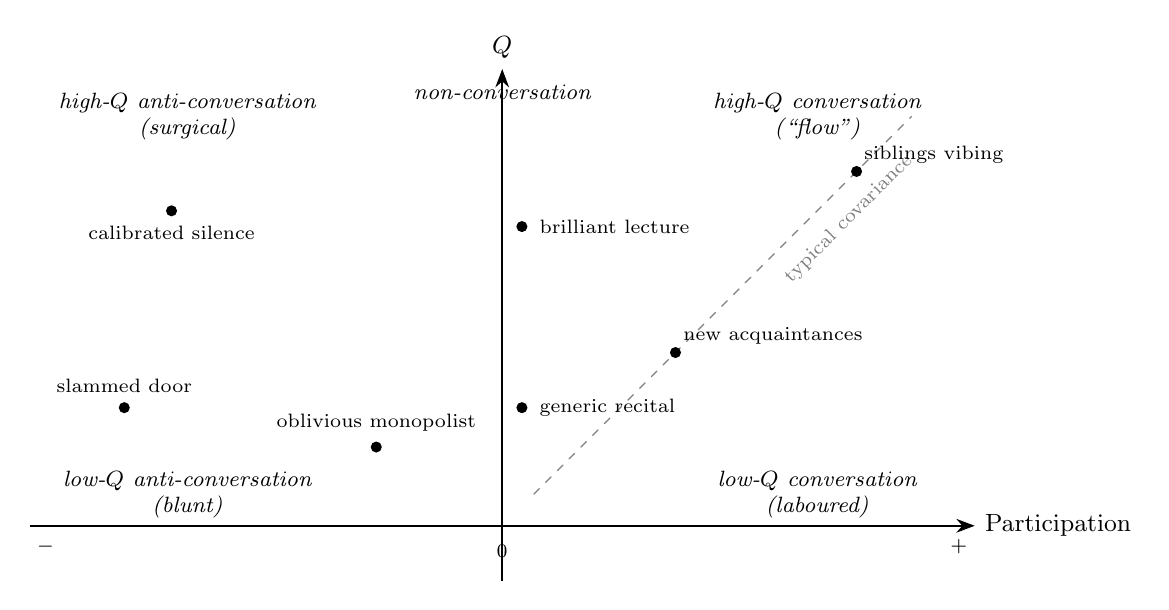
\begin{tikzpicture}[scale=1.0,>=Stealth]
    \draw[->,thick] (-6.0,0) -- (6.0,0) node[right] {\small Participation};
    \draw[->,thick] (0,-0.7) -- (0,5.8) node[above] {\small $Q$};
    \node[below] at (5.8,-0.05) {\scriptsize $+$};
    \node[below] at (-5.8,-0.05) {\scriptsize $-$};
    \node[below=2pt] at (0,-0.05) {\scriptsize $0$};
    % quadrant labels positioned in clear regions
    \node[align=center,font=\footnotesize\itshape] at (4.0,5.2) {high-$Q$ conversation\\(``flow'')};
    \node[align=center,font=\footnotesize\itshape] at (4.0,0.4) {low-$Q$ conversation\\(laboured)};
    \node[align=center,font=\footnotesize\itshape] at (-4.0,5.2) {high-$Q$ anti-conversation\\(surgical)};
    \node[align=center,font=\footnotesize\itshape] at (-4.0,0.4) {low-$Q$ anti-conversation\\(blunt)};
    \node[font=\footnotesize\itshape] at (0,5.5) {non-conversation};
    % diagonal
    \draw[dashed,gray] (0.4,0.4) -- (5.2,5.2);
    \node[gray,font=\scriptsize,rotate=45] at (4.4,3.9) {typical covariance};
    % example points -- labels positioned to avoid all collisions
    \fill (4.5,4.5) circle (2pt);
    \node[font=\scriptsize,above right=-1pt] at (4.5,4.5) {siblings vibing};
    \fill (2.2,2.2) circle (2pt);
    \node[font=\scriptsize,above right=-1pt] at (2.2,2.2) {new acquaintances};
    \fill (-4.2,4.0) circle (2pt);
    \node[font=\scriptsize,below=2pt] at (-4.2,4.0) {calibrated silence};
    \fill (-4.8,1.5) circle (2pt);
    \node[font=\scriptsize,above=2pt] at (-4.8,1.5) {slammed door};
    \fill (-1.6,1.0) circle (2pt);
    \node[font=\scriptsize,above=2pt] at (-1.6,1.0) {oblivious monopolist};
    \fill (0.25,3.8) circle (2pt);
    \node[font=\scriptsize,right] at (0.35,3.8) {brilliant lecture};
    \fill (0.25,1.5) circle (2pt);
    \node[font=\scriptsize,right] at (0.35,1.5) {generic recital};
  \end{tikzpicture}
  \caption{The two-axis space organising conversational moves. The horizontal axis is participation in the ARP contract, signed: positive for engagement, zero for non-engagement (lecture, monologue, ritual), negative for moves directed against the contract. The vertical axis is quality ($Q$), indexing the degree of compression of the three structural components. Typical conversational exchanges cluster near the dashed diagonal in the positive--positive quadrant. Off-diagonal cases are diagnostic of the orthogonality of the two axes.}
  \label{fig:plane}
\end{figure}

The positive--positive quadrant houses conversation proper. Most exchanges fall on or near the dashed diagonal: sincere participation tends to support model-building, which supports higher $Q$, which rewards continued participation. Pairs with deeply trained models of each other (siblings, close friends) occupy the upper-right region. New acquaintances who are genuinely engaging with each other occupy the lower-positive region, with $Q$ that typically rises across the exchange as their models build.

The zero-participation column houses non-conversational activities. These can be high-$Q$ (a brilliant lecture tailored precisely to the audience) or low-$Q$ (a generic recital), but they are not deficient conversations; they are different activities entirely. Speakers who attempt to import these activities into conversational contexts (the colleague who lectures at meetings, the relative who recites at family dinners) produce the experience of ``not really having a conversation''---an accurate phenomenology, on the present account.

The negative-participation quadrants house anti-conversational moves: moves that engage the ARP grammar specifically to attack or terminate it. The high-$Q$ region houses surgical anti-conversation: the calibrated non-receipt to a vulnerable disclosure, the precisely timed interruption, the pointed silence that exploits the partner's expectation of a receipt to wound them. The modelling is sharp; it is being used to harm the conversation precisely. The low-$Q$ region houses blunt anti-conversation: the slammed door, the unmodulated ``shut up,'' the storm-out. Termination without precision.

\subsection{Diagnostic off-diagonal cases}

Three cases illustrate the orthogonality of the axes.

\paragraph{The bookie's worse-offer} In adversarial negotiation, a party who has received a counter-offer sometimes responds with a worse offer than the original. The move is intelligible only because everyone knows the expected next move is a counter-counter that splits the difference. The bookie's worse-offer is a high-$Q$, positive-participation move: it demonstrates that the bookie has accurately assimilated the other party's position and expected response, and it weights the pivot toward aggression. The bookie remains on the contract; the cruelty is in the weighting, not the abandonment of the activity. This is different in kind from the bookie who says ``we're done here,'' which is a negative-participation move using the conversation to end it.

\paragraph{The calibrated silence} A partner makes a vulnerable disclosure. The expected receipt does not arrive. Instead, the second party produces a deliberate silence calibrated to the precise moment at which a receipt was expected, withholding the very response the partner's contribution required. This is a high-$Q$, strongly negative-participation move. The modelling is sharp---the silence is precisely timed---and the participation is sharply negative, because the silence is a move against the contract, intelligible only as a refusal of the receipt that was structurally invited. This is more wounding than a comparably long inattentive silence, because the inattentive silence is zero-participation while the calibrated silence is negative-participation. The sign matters even when the surface action (saying nothing) is the same.

\paragraph{The oblivious monopolist} A speaker holds the floor through extended turns, talks over TRPs, and pre-empts the other party's attempts to ARP. They are not, however, attacking the contract; they are simply not modelling the other party at all. Their occasional ``responses'' are mechanical pivots off keywords with receipts that don't show assimilation. This is a low-$Q$, low-or-negative-participation move depending on whether the monopolisation is incidental or directed. The partner withdraws---but, on the present account, withdraws differently than they would from the surgical anti-conversation case. The surgical case produces sharp injury; the oblivious case produces a kind of fog in which the partner cannot locate an adversary, only an absence.

The three cases together show that participation and $Q$ are genuinely orthogonal. A move can be sharply modelled and sincerely participating (the bookie), sharply modelled and anti-participating (the calibrated silence), or weakly modelled across a range of participation values (the monopolist). The plane is the right structure; a line is not.

\section{Why the ARP Cannot Be Derived from Any Single Parent Theory}\label{sec:against}

A natural defensive question is whether the ARP construct is genuinely new or whether it is a re-description, in new terminology, of phenomena already characterised within one of the parent literatures. I consider four candidate reductions.

\subsection{Is the ARP just interactive alignment with a public-verification step bolted on?}

Alignment as Pickering and Garrod describe it is a property of the dialogic state, not a property of any particular move. It does not pick out a position at which alignment is mutually verified. The ARP construct claims that alignment, however produced, must be periodically and publicly verified for grounded dialogue to proceed, and that the ARP is the move at which that verification occurs. The construct also picks out the $Q$ dimension, which is invisible to a pure alignment account: alignment as a state cannot distinguish high-$Q$ from low-$Q$ ARP-exchange, since both produce the same priming-based convergence. Alignment supplies conditions for ARPs; it does not constitute them.

\subsection{Is the ARP just Clark's contribution model with the acceptance phase moved earlier?}

The contribution model can accommodate the receipt component of an ARP, treating it as an anticipated acceptance. But it does not predict the structural coupling of receipt and pivot, and it does not pick out the participation axis as signed. In Clark's model, withdrawal of acceptance disrupts grounding, but the model does not distinguish zero-participation from negative-participation moves, which are phenomenologically distinct on the present account.

\subsection{Is the ARP just a collaborative completion that happens to continue past the completion point?}

Lerner and Hayashi are explicit that anticipatory completions terminate at the TCU boundary. The ARP is structurally distinct: the receipt is not necessarily a syntactic completion of the prior speaker's structure but a reformulation in the listener's terms, and the pivot is a new contribution by the second speaker rather than a continuation of the prior turn. The shared timing of high-$Q$ ARPs and anticipatory completions masks a different structural function.

\subsection{Is the ARP just a polite form of intrusive interruption?}

Intrusive interruption takes the floor without projection licensing and typically redirects the topic. The ARP takes the floor with projection licensing and continues the inferential trajectory. The same surface feature---second speaker beginning before first speaker has finished---supports an ARP if the onset is at the projected boundary and the continuation extends the inferential chain, and supports intrusive interruption if it is not and does not. The two are categorically distinct, and they sit in different regions of the participation axis: ARPs in positive participation, intrusive interruptions typically in zero or negative.

\section{Empirical Predictions}\label{sec:predictions}

I derive predictions along both axes. Predictions about the participation axis test the constitutive claim. Predictions about the $Q$ axis test the quality dimension. Several predictions are uniquely entailed by the integrated construct.

\subsection{Predictions about the participation axis}

\paragraph{P1. The folk taxonomy of communicative activities tracks the participation axis} Speakers' judgments about whether an exchange ``counted as a conversation'' should correlate with the proportion of turns that meet ARP criteria, controlling for total speaking time and turn count. Lectures, monologues, and rituals should score low on this proportion; conversations should score high. Speakers should reliably distinguish zero-participation activities from negative-participation episodes, even when both involve few ARPs, with the latter producing reports of being shut down or talked over rather than reports of having heard a lecture.

\paragraph{P2. Recovery asymmetry between zero and negative participation} Dialogic engagement should recover more readily from zero-participation interruption than from negative-participation interruption of equivalent duration. A pair whose conversation is interrupted by one party giving a brief lecture should resume conversation more quickly and at higher $Q$ than a pair whose conversation is interrupted by a comparable-length negative move (e.g., a sharp ``stop''). The sign of the participation move, not the duration of the non-ARP interval, is the relevant variable.

\paragraph{P3. Anti-conversational moves presuppose the contract} Negative-participation moves should be impossible (or perceived as misfires) in contexts where the ARP contract is not in effect. ``Stop talking'' as a hostile move requires a context in which someone was contributing to a conversation; it cannot be deployed in a context where no conversation was happening, since there is nothing to stop. This prediction is testable by examining the contexts in which negative-participation moves are produced and received as well-formed.

\paragraph{P4. Withdrawal under dominance is mediated by ARP-opportunity, not speaking time} In dyads where one party suppresses projection space, the other party's contribution rate should decline, mediated by reduced ARP opportunities rather than by reduced speaking time. Controlling for total available speaking time, parties denied projection space should still withdraw. Conversely, parties given ample speaking time but denied ARP opportunities (e.g., partners who reformulate everything themselves rather than allowing the addressee to do so) should also withdraw, despite having the floor. The prediction is testable with confederate paradigms in which speaking time and projection availability are independently manipulated.

\subsection{Predictions about the quality axis}

\paragraph{P5. $Q$ predicts the phenomenology of flow above and beyond density} Self-reported conversational flow should correlate more strongly with ARP $Q$ than with ARP density, in dyads matched on positive participation. Pairs producing many low-$Q$ ARPs should report less flow than pairs producing fewer but higher-$Q$ ARPs. The various Q-properties (pre-emption, succinctness, crystallisation, generativity, insight) may differentially predict flow, with crystallisation and insight expected to produce the strongest reactions because they deliver content the prior speaker had not produced themselves.

\paragraph{P6. $Q$ is relationship-dependent} ARP $Q$ between long-acquainted pairs (siblings, close friends, long-married partners) should exceed ARP $Q$ between matched strangers, in conversations of comparable topic and length. $Q$ within a developing relationship should climb across repeated encounters as mental models of the partner stabilise.

\paragraph{P7. Expert conversational partners produce elevated $Q$ with strangers} Interviewers, therapists, and similar trained roles should produce ARP $Q$ with strangers that is closer to the levels typical of close pairs, indicating that $Q$ is in part a trainable skill of rapid partner-modelling rather than purely a function of accumulated relational history.

\paragraph{P8. Receipt without pivot is distinct from pivot without receipt} Conversations rich in formulations but lacking pivots should be experienced as ``summarising,'' ``therapeutic,'' or ``passive''; conversations rich in pivots without receipts should be experienced as ``tangential'' or ``not listening.'' Only the integrated ARP should produce the flow phenomenology. This is operationalisable: confederates can be instructed to produce receipts without pivots, or pivots without receipts, with naïve participants' post-conversation ratings of flow, affiliation, and being-listened-to differing in the predicted directions.

\paragraph{P9. Q-properties may dissociate within speakers} Individual speakers should show stable profiles across the Q-properties, with some producing reliably succinct receipts but unimaginative pivots, others producing insightful pivots prefaced by laboured receipts, and so on. The dissociations should map onto recognisable conversational styles and should be detectable in longitudinal samples of a speaker's conversational behaviour with multiple partners.

\subsection{Predictions about interaction of the axes}

\paragraph{P10. High-$Q$ anti-conversational moves wound more than low-$Q$ ones} Calibrated silence after a vulnerable disclosure (high $Q$, strongly negative participation) should produce greater lasting damage to the relationship than a slammed door (low $Q$, strongly negative participation) of comparable surface duration. The combination of sharp modelling and negative participation is the most harmful region of the space.

\paragraph{P11. Developmental dissociation between participation and $Q$} Children should master entry into the ARP contract (positive participation) before mastering high $Q$. Component practices (collaborative completion, formulation, topic extension) should appear earlier in development, with their integration into single ARP moves following theory-of-mind consolidation. $Q$ should continue to develop throughout life, with adults remaining capable of substantial improvement in conversational skill.

\subsection{Predictions distinctive of the integrated construct}

P2, P3, P4, P8, P9, and P10 are the predictions that most distinctively follow from the integrated ARP construct and the two-axis structure. Interactive alignment alone does not predict the signed structure of the participation axis, nor the recovery asymmetry between zero and negative interruption. The contribution model does not predict the structural coupling of receipt and pivot, nor the distinct phenomenology of receipts-without-pivots and pivots-without-receipts. Collaborative completion theory does not predict the $Q$ dimension or its sub-properties. Dominance theory does not predict that ARP-opportunity rather than speaking time mediates withdrawal. The plane structure, with its diagnostic off-diagonal cases, is uniquely entailed by the constitutive view.

\section{A Methodological Programme}\label{sec:methods}

\subsection{Coding}

A coding scheme for ARPs requires identifying the three structural components in each move: evidence of assimilation (whether pre-emptive or post-completion), a receipt that reformulates the prior contribution, and a pivot that extends the inferential chain. $Q$ can be coded along its sub-dimensions: pre-emption of receipt (does it land before or after the prior TRP?), succinctness (length ratio of receipt to relevant portion of prior contribution), crystallisation (does the prior speaker ratify the receipt as more precise than their own articulation?), generativity (does the pivot open new inferential territory or merely restate?), and insight (is the pivot recognised by the prior speaker as revealing something the assimilation produced in the moment?). The participation axis is coded by the sign and direction of each move's relation to the ARP contract. Inter-rater reliability should be established on a calibration corpus before substantive analysis.

Existing conversational corpora (Switchboard, CallHome, the British National Corpus's spoken section, the Saarbrücken Spontaneous Speech corpus) supply candidate material. Tests of $Q$-dependent predictions require new recordings with post-conversation flow ratings and, ideally, relationship information about the dyads.

\subsection{Experimental manipulation}

Confederate paradigms permit direct tests along both axes. To test predictions about the participation axis (P2--P4), confederates can be instructed to: (a) produce ARPs at a controlled rate; (b) shift into a zero-participation mode (deliver a lecture-like segment); (c) shift into a low-$Q$ negative-participation mode (blunt termination); or (d) shift into a high-$Q$ negative-participation mode (calibrated non-receipt at a vulnerable moment, as judged by the prior content). Outcome measures include the naïve participant's contribution rate, the rate at which they attempt ARPs that are pre-empted, post-conversation ratings, and recovery time when the confederate returns to ordinary engagement.

To test $Q$ predictions (P5--P9), confederates can be trained to produce ARPs with controlled profiles across the Q-sub-dimensions: pre-emptive vs.\ post-completion receipts, succinct vs.\ verbose receipts, crystallising vs.\ literal receipts, generative vs.\ restating pivots. The differential prediction of flow, affiliation, and being-listened-to should map onto the sub-dimensions.

\subsection{Self-report}

Validated flow scales \citep{JacksonMarsh1996} adapted for dyadic conversation can serve as the subjective endpoint. Care must be taken to distinguish flow from affiliative warmth, which is empirically correlated but theoretically distinct: $Q$ should predict flow more strongly than warmth.

\subsection{Neural measures}

Hyperscanning paradigms \citep{Stephens2010,Liu2017} measure inter-brain coupling during conversation. P5 predicts that coupling indices should peak around ARP boundaries and should be higher for high-$Q$ than for low-$Q$ ARPs. P10 predicts that the neural response to high-$Q$ negative-participation moves should differ from the response to low-$Q$ ones in ways that index the asymmetric harm.

\subsection{Development}

Tests of P11 require longitudinal child--child and child--adult conversational data. Existing corpora in CHILDES supply some material; targeted longitudinal recording in middle childhood (ages 6--10) would supply the rest. The prediction is that entry into the ARP contract precedes the maturation of $Q$, with $Q$ continuing to develop into adolescence and adulthood and the various Q-properties potentially maturing at different rates.

\section{Discussion}\label{sec:discussion}

\subsection{Theoretical implications}

If the ARP is the constitutive unit of conversation, several consequences follow.

First, the folk taxonomy of communicative activities is theoretically principled rather than incidental. We have separate words for lecture, monologue, ritual, conversation, and argument because they are different activities, distinguished by the presence, absence, or inversion of ARP-exchange. The taxonomy is empirically tractable on the present account: each activity has a predictable signature in the two-axis space.

Second, the parent literatures' findings are partially absorbed and partially extended. Projection, collaborative completion, alignment, grounding, and the dominance--withdrawal link are all preserved as substantive findings, but they are reorganised. They describe features of, conditions for, or violations of a single underlying mechanism rather than independent phenomena. Several predictions of the parent theories are sharpened: alignment without ARP-based verification should be unstable; grounding through pre-emptive receipts should be quicker than through delayed acceptance; dominance-induced withdrawal should be mediated by ARP-opportunity specifically.

Third, the construct supplies a vocabulary for clinical and applied work that the parent literatures have not provided in unified form. Conversational therapy, coaching, mediation, and interview training all attempt to cultivate something the present account names: high-$Q$ positive participation. Negative-participation interventions (boundary-setting, terminating abusive exchanges) acquire a structural account of why they work and when they backfire. Conversational dysfunctions associated with autism spectrum conditions, certain personality disorders, and dementias can in principle be located in the plane, with different conditions producing characteristic distortions of $Q$, of participation, or of the integration between them.

Fourth, the constitutive claim invites re-examination of communicative practices that wear conversational clothing but may not be conversations on the present account: corporate meetings, performative dialogue, much political debate, and certain forms of mediated exchange (broadcast interviews, scripted podcasts). The empirical question is whether ARP-exchange is occurring, and the prediction is that the phenomenology of these exchanges---often reported as performative, draining, or unsatisfying---will track the absence of ARP-exchange even where the surface form mimics it.

\subsection{Limitations}

The construct is functionally defined, and operationalisation will need to avoid circularity, particularly for the pivot component and for $Q$. The methodological programme is designed to address this through converging measures, but the construct's empirical utility depends on the success of operationalisation.

The Q-properties enumerated in Section~\ref{sec:plane} are illustrative rather than exhaustive. Future work may identify additional properties that drive compression, and the construct is explicitly open to such extensions. The risk is that the openness becomes a license for post-hoc accommodation; the methodological programme should pre-register the Q-properties measured before each empirical test.

The present analysis is restricted to dyadic conversation. Multi-party interaction introduces complications: when more than one listener might claim a receipt, the structure of ARP rights becomes contested, and the move may function partly as a bid for affiliation with the prior speaker against other listeners. Whether multi-party ARPs serve this affiliative function in addition to their grounding function is an open empirical question.

The relation between ARPs and disagreement requires careful handling. Receipts presuppose accurate assimilation but not agreement. An ARP that accurately formulates a partner's projected conclusion in order to argue against it is still an ARP. Whether disagreement-pivoting ARPs produce flow phenomenology comparable to agreement-pivoting ARPs is empirically open; the answer will inform what flow itself is.

The claim of structural necessity in Section~\ref{sec:nontrivial}---that the three components of an ARP are mutually constitutive rather than merely co-occurring---is a strong hypothesis. The weaker claim, that the three are temporally distinct subprocesses unfolding rapidly within a single conversational position, is the principal alternative. Neural and chronometric measures can adjudicate.

The signed participation axis treats the boundary between zero and negative participation as principled, but real exchanges contain gradations. A long pedagogical aside in a conversation may shade from positive into zero participation; an inattentive silence may shade into a calibrated one. The construct treats these as transitions through the space rather than as ambiguous categorisations, but the empirical study of such transitions will be more methodologically demanding than the study of clear cases.

\subsection{Conclusion}

The Assimilate--Receipt--Pivot is not, in any of its components, a novel observation. Projection, completion, alignment, grounding, and the consequences of their failure have each been studied extensively, by traditions with strong empirical foundations. The contribution offered here is the proposal that one frequently occurring move performs all of these functions simultaneously, that this move constitutes conversation as a distinct communicative activity, that the moves that surround it---non-conversational activity, anti-conversational attack, gradations of compression quality---occupy a principled two-axis space, and that the standard phenomenology of dialogic experience sorts into this space in ways the parent literatures, severally, do not predict. The construct is offered as a hypothesis. Its empirical evaluation is open.

\medskip
\noindent\textbf{Acknowledgements.} Anthropic's Claude AI (Opus 4.7) software was used in preparing this manuscript.

\bibliography{arp}

\end{document}
